%! program = pdflatex

\documentclass[11pt]{report}
\usepackage{geometry}
\geometry{a4paper}
\usepackage[parfill]{parskip}
\usepackage[T1]{fontenc}
\usepackage{graphicx}
\usepackage{amssymb}
\usepackage{epstopdf}
\usepackage{framed}

% \DeclareGraphicsRule{.tif}{png}{.png}{`convert #1 `dirname #1`/`basename #1 .tif`.png}

\sloppy

\usepackage[colorlinks=true, pdfstartview=FitV, linkcolor=blue,
            citecolor=blue, urlcolor=blue]{hyperref}

\setlength{\parindent}{0pt}
\setlength{\parskip}{2ex plus 0.5ex minus 0.2ex}

\title{Introduction to Access Management \\
using Oracle Access Manager}
\author{Horst Kapfenberger}
\date{March 14, 2016}

\begin{document}

\maketitle

\begin{abstract}
    Introduction to Access Management in the area of Information
    Technology.  Description of user authentication, authentication
    factors and methods.
   
    Further explanation is done on the basis of an established
    proprietary software, \emph{Oracle Access Management Access
    Manager}.
    
    Detailed description of the Single-Sign-On process and the
    implementation in the considered product.

    Sample messages and software configuration excerpts are added.
\end{abstract}


% \newpage

\tableofcontents

%!TEX root =  main.tex

\section{Access Management}

\subsection{Controlling Access}

What is Access Management in IT\@?

In the area of information technology the subject ``Access Management'' 
has several subareas

\begin{itemize}
    \item Application Security: restrict users and programs
    \item User Productivity: providing users with ease access to their needs
    \item Middleware technology
\end{itemize}



\subsection{In Real Life: Border Controls}

A good comparison to illustrate the main characteristics of
authentication is \emph{border control}. That one you'll most often find
on airports or on the actual boarder between countries\footnote{There
was a time you had to leave \emph{Schengen Area} to find this seldom
experience, nowadays there seems to be an inflation of borderline
checks.}.

You leave one domain, or more important: you enter another domain. 
A domain that has a certain definition, borders, and authorities that 
execute policies (for good and for bad, however).  Those brave officers 
want you to identify yourself --- your job is to provide them data, exact 
and distinct data and some prove that you tell the truth.

The data is usually good enough to identify you among all human beings.
That quality of your prove must satisfy the procedure of those border
checks. With a valid passport you own a document from a common trusted
authority that covers this.

\begin{enumerate}
    \item[-] identifying you among all others and (identification)
    \item[-] prove the correctness of this statement (authentication)
\end{enumerate}

For you, as the traveler, the desired outcome of this procedure is your
valid entry without much delay.


\subsubsection{Alternative Flows}

Thinking more general, what other situations in or outcomes of this
situation are possible?

\begin{itemize}
    \item[-] you could pretend to be another person, perhaps from another 
        country
    \item[-] you could sneak in the country, preventing any check
    \item[-] you could mix you passport by mistake in the cafeteria next 
        to the borderline.  You enter the country with a different identity 
        without knowing
    \item[-] your passport is expired and you are not allowed to enter the 
        country
    \item[-] etc.
\end{itemize}

All those situations have a direct mapping to use cases in the IT world.

\subsubsection{Not Authorized}

One more thing is in common: it is not checked what exactly you are
allowed to do (in the country or domain). There might be a rough
categorization by authentication, like people from country X would also
need a visa and people from country Y are not allowed at all to enter.
But this is not the place where a work or residence permit would be
checked (as far as I know).

Using our vocabulary, we are \emph{authenticated} but no authorization
check has been done.


%!TEX root =  main.tex

\section{Authentication}

\subsection{What's Authentication}

\emph{Authentication} is the act of confirming the truth of an attribute
of a single piece of data (a datum) claimed true by an entity. In
contrast with \emph{identification} which refers to the act of stating
or otherwise indicating a claim purportedly attesting to a person or
thing's identity, authentication is the process of actually confirming
that identity.


\subsection{Authentication Factors}

The ways in which someone may be authenticated fall into three
categories, based on what are known as the factors of authentication:
something the user \emph{knows}, something the user \emph{has}, and
something the user \emph{is}.

Each authentication factor covers a range of elements used to
authenticate or verify a person's identity prior to being granted
access, approving a transaction request, signing a document or other
work product, granting authority to others, and establishing a chain of
authority.


The three factor types and some of elements of each factor are:

\begin{description}

    \item \emph{knowledge factor}: something the user knows, e.g.\ a 
        password, Partial Password, pass phrase, or personal identification 
        number (PIN), challenge response (the user must answer a question, 
        or pattern), Security question

    \item \emph{ownership factor}: something the user has (e.g.\ wrist band, 
        ID card, security token, cell phone with built-in hardware token, 
        software token, or cell phone holding a software token)

    \item \emph{inherence factor}: something the user is or does (e.g.\ 
        fingerprint, retinal pattern, DNA sequence (there are assorted 
        definitions of what is sufficient), signature, face, voice, 
        unique bio-electric signals, or other biometric identifier)

\end{description}


For authentication to well-secured systems elements from at least two,
and preferably all three, factors should be verified.


\subsection{Authentication Methods}

TODO



%!TEX root =  main.tex

\section[Product Overview]{Product Overview}

\subsection{Access Management Suite}

Around 2010 Oracle corporation aquired a docen software vendors and
technology companies in the identity and access management market. Among
them were some niche players and also leaders, like Sun Microsystems
with several active products and a stable user base.

Developing a portfolio of twenty specialized systems to two or three
tightly integrated solutions definitely the overal plan, but not every
step is set straight on that path, looking at the footsteps we see
sometimes.

Next to the Identity Management Suite the Access Management Suite is the
second major product group, where the collected technologies deal with
run-time evaluation of user or system access.

The Access Manager itself is the heart of Suite, where other products or
new feature sets have been integrated or merged into.

\begin{itemize}
    \item Access Manager
    \item Identity Federation
    \item Security Token Service
    \item Mobile and Social
    \item Adaptive Authentication Service
    \item OAuth Services
    \item Identity Context
\end{itemize}


\paragraph{Access Management Access Manager}

As the central part of the suite, Access Manager delivers the
adminstrative user interface. All authentication mechanisms are defined
here and components and processes can be activated or cut-off in the
admin user interface. Business applications can be registered and and
external data sources with user data are connected.

Distributed components, the policy enforcement points, are located
closer to the protected business applications and request authentication
and authorization information from the central access server over
encrypted channels.


\paragraph{Identity Federation}

While Access Manager takes care of a single domain (or multiple but
independent domains), Identity Federation helps to connect domains
(e.g.\ two organizations with integrated business activities).  In each
activity the roles and responsibilities are well defined. Indentity
Federations supports SAML and OpenID\@.

\paragraph{Security Token Service}

Token validation and generation to facilitate access to services across
security domains and beyond organizational boundaries. Essentially the
service acts as a trust-broker that receives and validates client
requests and generates appropriate tokens for a requested resource.

\paragraph{Mobile and Social}

Mobile (for mobile devices): integrate iOS and Android mobile devices,
policy enforcement on those devices, single-sign-on for mobile apps and
browser based access, SDK on mobile devices.

Social (for social services): integrate authentication, policies for
several social services available on Internet.


\paragraph{Adaptive Authentication Service}

Real-time and batch risk analytics to prevent fraud and misuse, risk
based authentication, additional authentication methods, like
One-Time-Passwords (OTP).


\paragraph{OAuth Services}

OAuth 2.0 authentication client and server. Manage access control over
domain borders.


\paragraph{Identity Context}

Enable dynamic adation of permissions based on user related data, like
location, last transactions, third party informations, other assigned
permissions, etc.


This document covers topics from Access Managament Access Manager only.

% vi:set lbr breakindent:

%!TEX root =  main.tex

\section{Access Manager}

\subsection{Overview}

You can think of Access Manager as a general gate, in front of all your
applications, that each request has to pass. It ensures that only
authenticated requests are allowed to pass to the business application
that you are protecting.

For public accessible areas the authentication check is disabled. In
addition you can also skip auditing in this area, in case the data would
not be used anyway.

The session of an authenticated user defines the access and is protected 
agains external changes. The \emph{ticket} or the \emph{single sign on 
session} is stored central as well on the client (using cookies).

The boundaries of the single-sign-on session can be defined by domain
and subdomain namespaces. However this will only be enforced for
integrated applications.

Each session has set a \emph{general time-out} and an \emph{inactivity
time-out}. The general time out will close the session and force a
reauthentication, no matter if there is currently any activity ongoing
or not. Default value of this general time-out is 24 hours. The
inactivity time-out is set to a shorter period, depending on the
customer needs and security level.

Integrated applications often require an application session as well,
where user data is attached to. This session information is not touched 
by Access Manager.


The \emph{integration} of an application is relative simple exercise, since we
essentially remove functionality and code. In particular the login and
logout functionality is removed. Instead of returning an application
login page, the application can take the attached information like user
name, user ID, or roles, and continue with the transaction.

The logout link or button of the business application will remain on the
user interface. The business application will just redirect the user to
the general logout URI, which will trigger the necessary logout
callbacks to the used business applications. So the user sessions will
savely be closed on a general logout. However, as before this is
triggered when the user actively executes a logout.

The individual implementations of the user login and logout are removed
from applications during integration. Only authenticated requests can
reach the application from now on. While an authorization policy
enforcement is available and recommended, other products of the suite
may be necessary to cover different authorization requirements.



% ====================================================================

\section{Components of Access Manager}

In the following pages I will explain what parts or topics Access
Manager consists of and what the are good for:

\begin{itemize}
    \item Access Server
    \item Application Domains and Resources
    \item Identity Store
    \item Session Store
    \item Policy Enforcement Points: Agents
    \item Webgate Agent
    \item SSO Cookies
    \item Credential Collector
    \item Certificate Validation and Revocation
\end{itemize}




\subsection{Access Server}

The Access Server is the \emph{backend runtime component} that serves
requests of the \emph{Policy Enforcement Points}. It is implemented as
J2EE service and Oracle supports Oracle WebLogic and IBM WebShpere as
application servers. In WebLogic the services are deployed to one or
more managed servers grouped in a WebLogic cluster.  Most of the
interfaces and protocols are based on open standards, an exception here
is the propriary protocol to the policy enforcement points, called OAP
(Oracle Access Protocol).

The configuration can be done using the web user interface 
\emph{OAMConsole}, hosted on the WebLogic Admin Server. Many features
can also be configured using shell scripts or the WebLogic scripting
environment WLST\@. The substantial configuration is persisted as XML
file. Bindings and policies are stored in the relational database base
schema.


\subsection{Application Domains and Resources}

The value of an production access system, comes from the integrated
business applications. Therefore the management of those business
applications and their policies is a central area in Access Manager.

Applications are mapped to application domains. This mapping can be done  
as an one-to-one relation, but also other transformations are possible,
as long as it helps the operational team to treat the integration as one
consistent block of applications, which is integrated or maintained at
once.

Each application domain consists of multiple resources. A resource can
be seen as an entitlement in the application domain. Since all resources
are expressed as \emph{Uniform Resource Identifier (URI)}, Access
Management uses the URI component \emph{path} and optionally \emph{query} and
\emph{fragment} as resource identifier.

Example resource identifier: \verb|/orders/**|



\subsection{Identity Store}

To execute the main feature of Access Manager, the authentication, we
need at least one set of identities that are allowed to authenticate.
This set must be stored in a supported directory server and should be
\emph{close} to Access Manager, in operational and data ownership
perspective.

Access Manager will read from and write to this identity store. The
required initial information in the store is the user login and some
status information of the user account.

Access Manager stores additional runtime data attached to the user
information.

Optional information that can be stored in the identity store can be
\emph{user credentials}, \emph{user roles}, etc.

In case you deploy \emph{Access Manager} with \emph{Oracle Identity
Manager} the directory is automatically populated and acts as a data hub
between Identity and Access Management.


\subsection{Session Store}

We already mentioned where user sessions are stored. But let's have a
closer look here.

For Access Manager it is essential to have clear accounting of active
user sessions, with additional information attached to them:

\begin{itemize}
    \item when did the session start
    \item timestamps used for time-outs
    \item authentication method used
    \item current and original authentication levels
    \item reference to identity store
    \item location (if applicable)
\end{itemize}

This information must be served quickly with high availability
requirements. Access Manager maintains this list in Coherence.

\begin{framed}
    Oracle Coherence is a proprietary in-memory data grid, that improves
    performance, scalability and reliability compared to relational
    databases. It can be used as an persistence system or as a caching
    method in combination to relational database system.
    
    Coherence was developed by \emph{Tangosol Inc.}, which was acquired 
    by Oracle Corporation in 2007. Several Oracle applications, like 
    Access Manager or SOA, use Coherence.
\end{framed}

The Access Manager admin interface \emph{oamconsole} comes with a
feature for querying and maintaining the session list.

The session information placed at the client side is described in the
section Cookies.


\subsection{Policy Enforcement Points: Agents}

The Policy Enforcement Points are the components actively asking Access
Manager for user access. They act as gatekeeper to the business
applications.




\subsection{Webgate Agent}

TODO


\subsection{SSO Cookies}

TODO


\subsection{Credential Collectors}

TODO


\subsection{Certificate Validation and Revocation}

TODO


\section{A Sample Use Case}

Let's make one assumption --- to simplify our examples: the applications
we are dealing with are web applications, to be more exact: the user
interface is rendered in a standard conform Internet browser.

There are ways to integrate legacy applications, however more analysis
work has to be done beforehand.

For web applications, the transport and integration protocol is HTTP or
HTTPS\@. Before our integration, the business application acts a as a
stand-alone application, in respect of the user session. An application
login page is presented to the user, in case the user has no active
session. After some work the user may log out or the session will be
finaly terminated by a time out (usually most of the user sessions end
with time-outs). Both session related actions, login and logout are
under control of the business application.

The implementation of the login functionality is critical, it is
critical in mutiple ways:

\begin{itemize}
    \item run time errors may block the whole business application
    \item often an external system call is needed, the response data 
        and its interpretation is not obvious or may change over time
    \item accounts may be locked in different ways, what shall be the 
        user error message?
    \item the business application (perhaps a 3rd party application) 
        needs to deal with user passwords
\end{itemize}

Dealing with all those challenges, a centralized solution like a
directory server, feels again like a redundant and error prone approach.
Quite often it also becomes a dangerous approach, when one of the
business applications or an operational tool is lacking the last
encryption method and sends plain text or it logs one attribute more
then it should (yes login credentials is not an uncommon problem).







\emph{User opens resource (URI) to start a system transaction}

So our start point is a user request for a resource, let's say a the first webpage of a customer maintenance workflow. The webpage is the resource the user requests. Our hypothetical system feature has two UI screens:

\begin{itemize}
    \item Customer search by account id
    \item Customer details screen
\end{itemize}

Access Management's webgate component is attached to the reverse proxy of the business application and inspects every request. The inspection starts like this:

New request 


\section{Sample Configuration}


% vi:set lbr breakindent:

%!TEX root =  main.tex

\chapter{Miscellanies}


\subsection{Authenticated Request}

An authenticated user requests a resource. Webgate has sucessfully verified the
request and added the user identifier (\verb|OAM_REMOTE_USER|) and domain
(\verb|OAM_IDENTITY_DOMAIN|). The request is now passed to the upstream system.

\scriptsize
\begin{verbatim}
Hypertext Transfer Protocol
    GET /cs/resources/yui/treeview/assets/treeview-core.css HTTP/1.1
        [Expert Info (Chat/Sequence): GET /cs/resources/yui/treeview/assets/tre
                eview-core.css HTTP/1.1
            [Message: GET /cs/resources/yui/treeview/assets/treeview-core.css 
                HTTP/1.1]
            [Severity level: Chat]
            [Group: Sequence]
        Request Method: GET
        Request URI: /cs/resources/yui/treeview/assets/treeview-core.css
        Request Version: HTTP/1.1
    Host:ucmdmsint.example.com
    User-Agent:Mozilla/5.0 (X11; Linux x86_64; rv:27.0) Gecko/20100101 Firefox/
                27.0 Iceweasel/27.0a2
    Accept:text/css,*/*;q=0.1
    Accept-Language:en-US,en;q=0.5
    Accept-Encoding:gzip, deflate
    DNT:1
    Referer:https://ucmdmsint.example.com/cs/idcplg?IdcService=GET_DOC_PAGE&Act
                ion=GetTemplatePage&Page=HOME_PAGE
    Cookie:IntradocAuth=NTLM; IdcLocale=English-US; IntradocLoginState=1; JSESS
                IONID=Q5cFSz0FXpYfHKTyyYvdrnjHGKw9jQLXRw0w0wbsTMj1yRC9m1bm!-197
                112114!-1961464539; _WL_AUTHCOOKIE_JSESSIONID=rcC0mwhZjCRvXDuC5
                3H6; IdcTimeZone=Europe/Vienna
    If-Modified-Since:Thu, 16 Feb 2016 15:28:49 GMT
    Cache-Control:max-age=0
    OAM_REMOTE_USER:KAPFENHO
    OAM_IDENTITY_DOMAIN:OIMIDStore
    ECID-Context:1.004vUS6Q5_AFo2wQcEiOPL0003SV00003c;kYjE1ZDLIPIRj3RSj2TPnVPTm
                JPPnV9UpPRBoITP_MTQ_NVBXJVS_KVSj4US_LQTdLRTh3RRmLQBZJVS
    Connection:Keep-Alive
    WL-Proxy-SSL:true
    X-Forwarded-For:192.0.2.16
    WL-Proxy-Client-IP:192.0.2.132
    Proxy-Client-IP:192.0.2.132
    WL-Proxy-Client-Port:30979
    X-WebLogic-KeepAliveSecs:30
    X-WebLogic-Request-ClusterInfo:true
    x-weblogic-cluster-hash:dZbfyq4+X4kn1DYr6dYHPPOWqpk
    
    [Full request URI: http://ucmdmsint.example.com/cs/resources/yui/treeview/a
                 ssets/treeview-core.css]
    [HTTP request 2/10]
    [Prev request in frame: 62]
    [Response in frame: 135]
    [Next request in frame: 160]
\end{verbatim}
\normalsize

\newpage

\begin{figure}
    \centering
    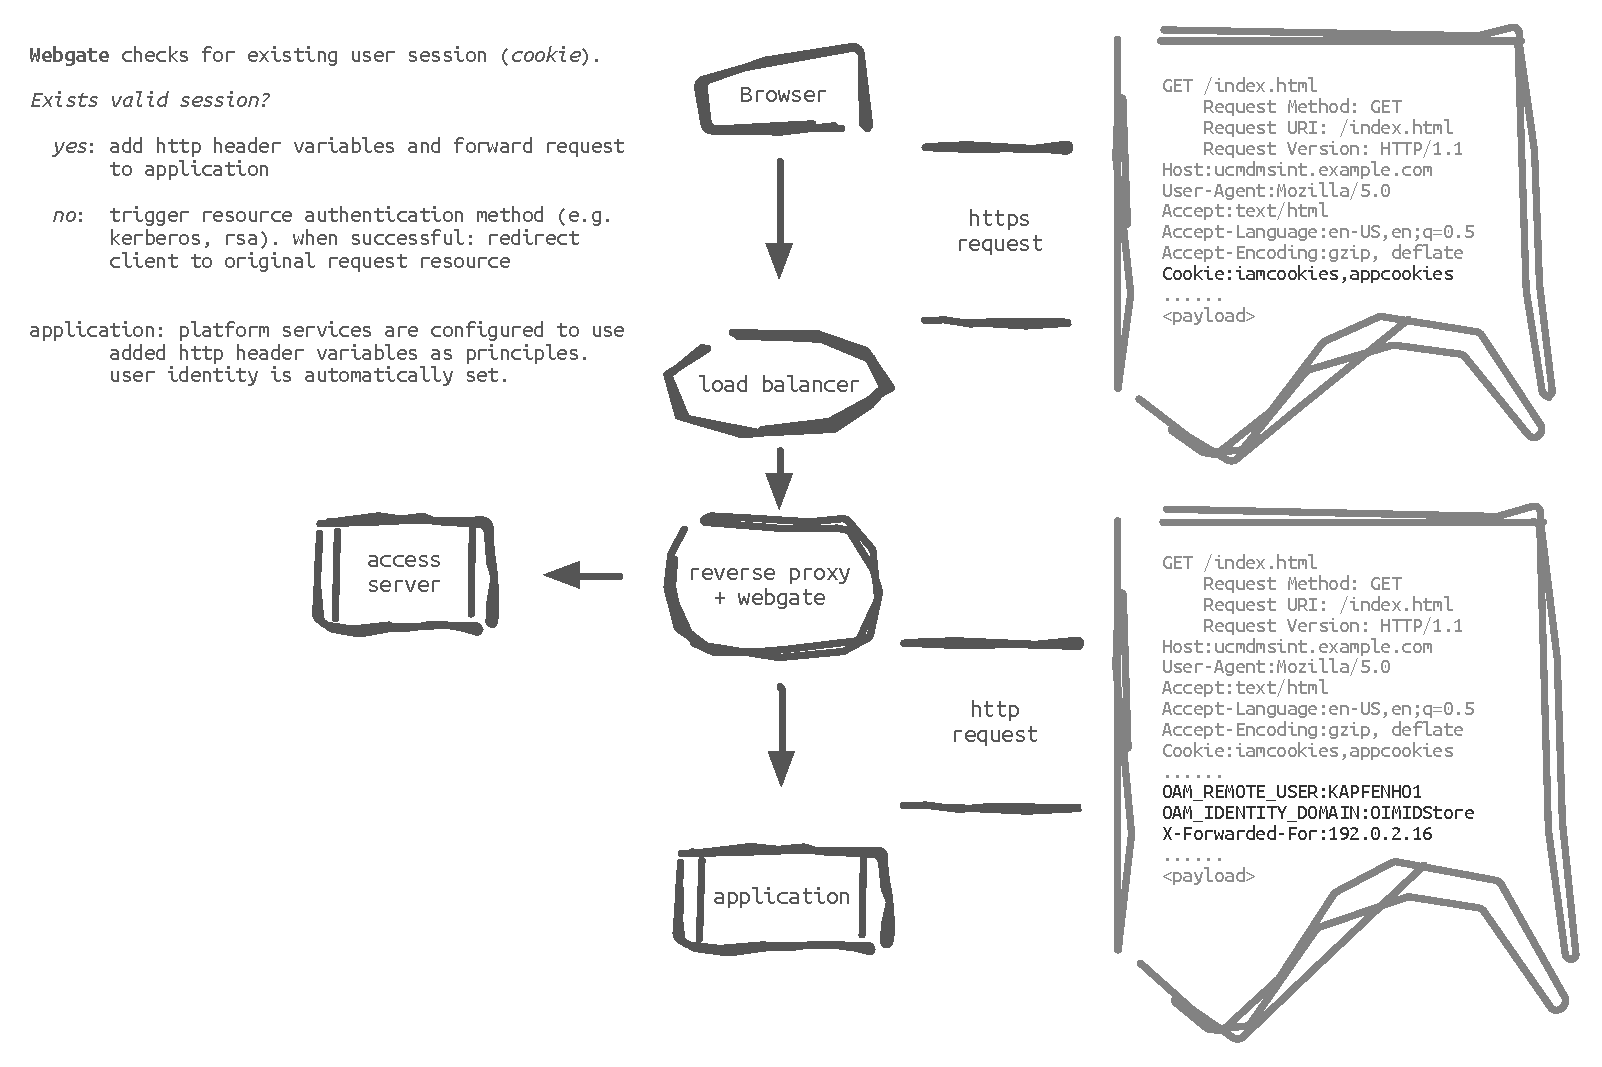
\includegraphics[width=1\textwidth]{diag/msgdiag}
    \caption{Login process with messages}
\end{figure}


\begin{figure}
    \centering
    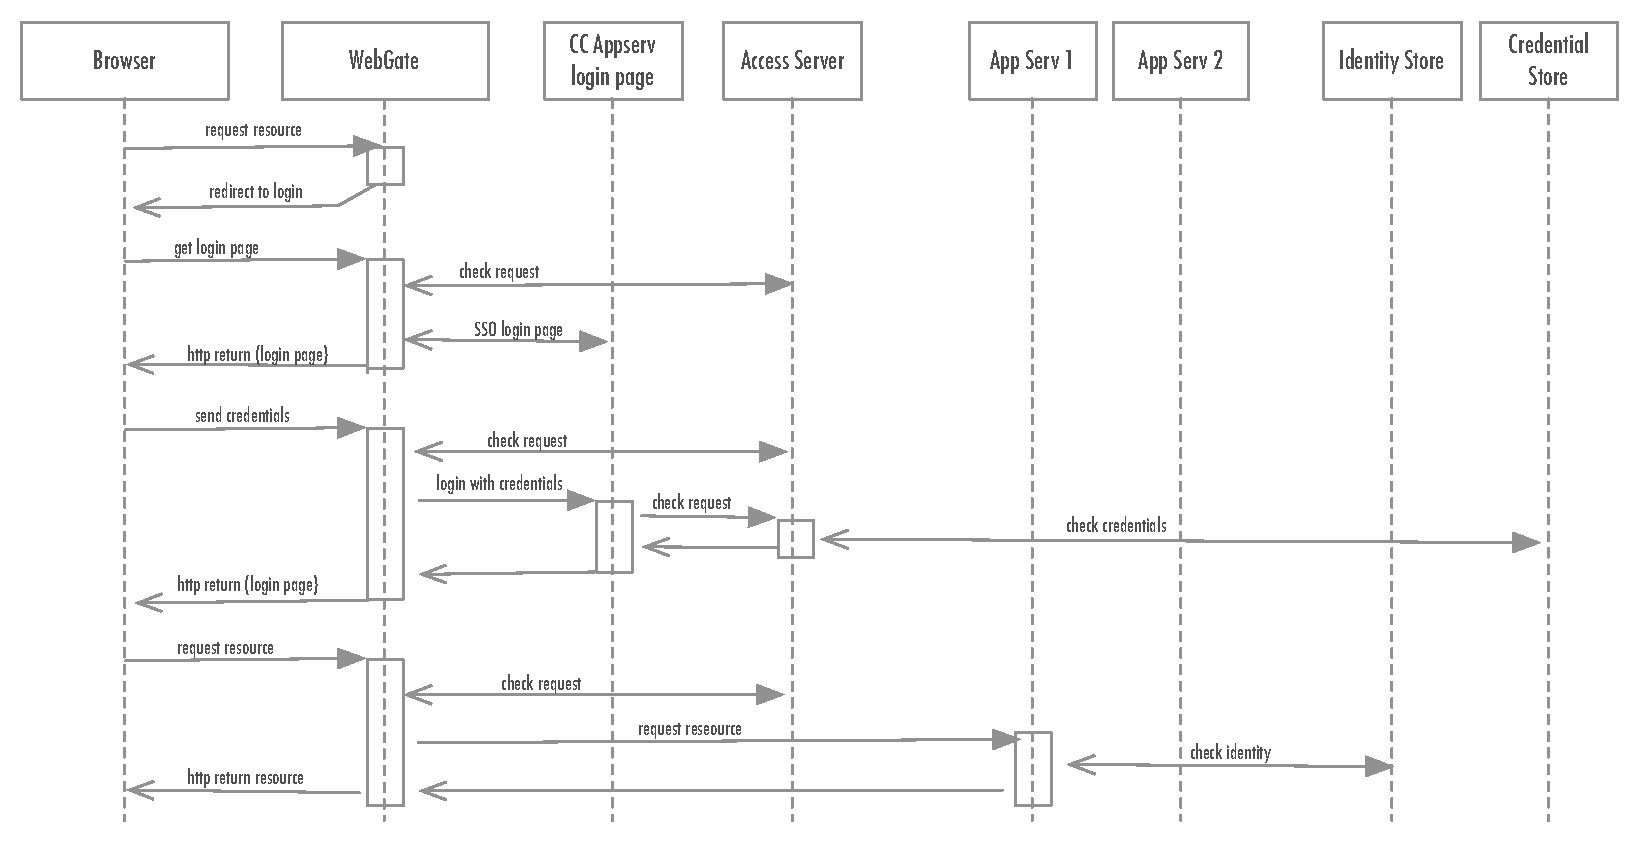
\includegraphics[width=1\textwidth]{diag/seqdiag}
    \caption{Sequence diagram of SSO login process}
\end{figure}


% vi:set lbr breakindent:


\bibliographystyle{plain-annote}
\bibliography{mybibliography}

\end{document}
